%\begin{savequote}[8cm]
%Far out in the uncharted backwaters of the unfashionable end of the western spiral arm of the Galaxy lies a small unregarded yellow sun. Orbiting this at a distance of roughly ninety--two million miles is an utterly insignificant little blue green planet whose ape--descended life forms are so amazingly primitive that they still think digital watches are a pretty neat idea.
%  \qauthor{--- D. Adams, The Hitchhiker's Guide to the Galaxy}
%\end{savequote}

\chapter{Introduction}\label{ch:1-intro}

\minitoc

How do you design and assemble something on the nanoscale? When working with everyday objects on the macroscale, it is easy to pick the building blocks you want and attach them where you want them to be. However, for nanoscale objects, it is difficult to have that level of top--down control. Instead, more success has been had by imitating nature and letting the building blocks assemble themselves. After millions of years of evolution, nature has the advantage. This thesis will cover novel methods and tools to design such self--assembling nanostructures.

\section{Background}
I am pursuing my graduate studies in Condensed Matter Physics as an Early--Stage Researcher, part of a Marie Skłodowska-Curie Innovative Training Network called \emph{DNA--Robotics}\footnote{\url{https://dna--robotics.eu/}, grant agreement number 765703}. The network consists of leading European DNA nanotechnology research groups and was formed with the goal of creating a unified framework for integrated biomolecular robotics \cite{dnaroboticsResearch}.

My position, in particular, is assigned to develop standardised techniques for the design and self--assembly of the nanorobotic modules \cite{dnaroboticsESR12}. The original design proposed for the robotic modules was to use cubic DNA origami modules, as shown in Figure \ref{fig:dnaRoboticsHeader}, but the network also investigated using interacting vesicles as the basic modules. Other Early--Stage Researchers within the network are developing such modules with either sensor, actuation or signal processing capabilities. The motivation for developing standardised modules is that, when proven to work, they can be reused in new designs, saving development time and resources.

\begin{figure}
    \centering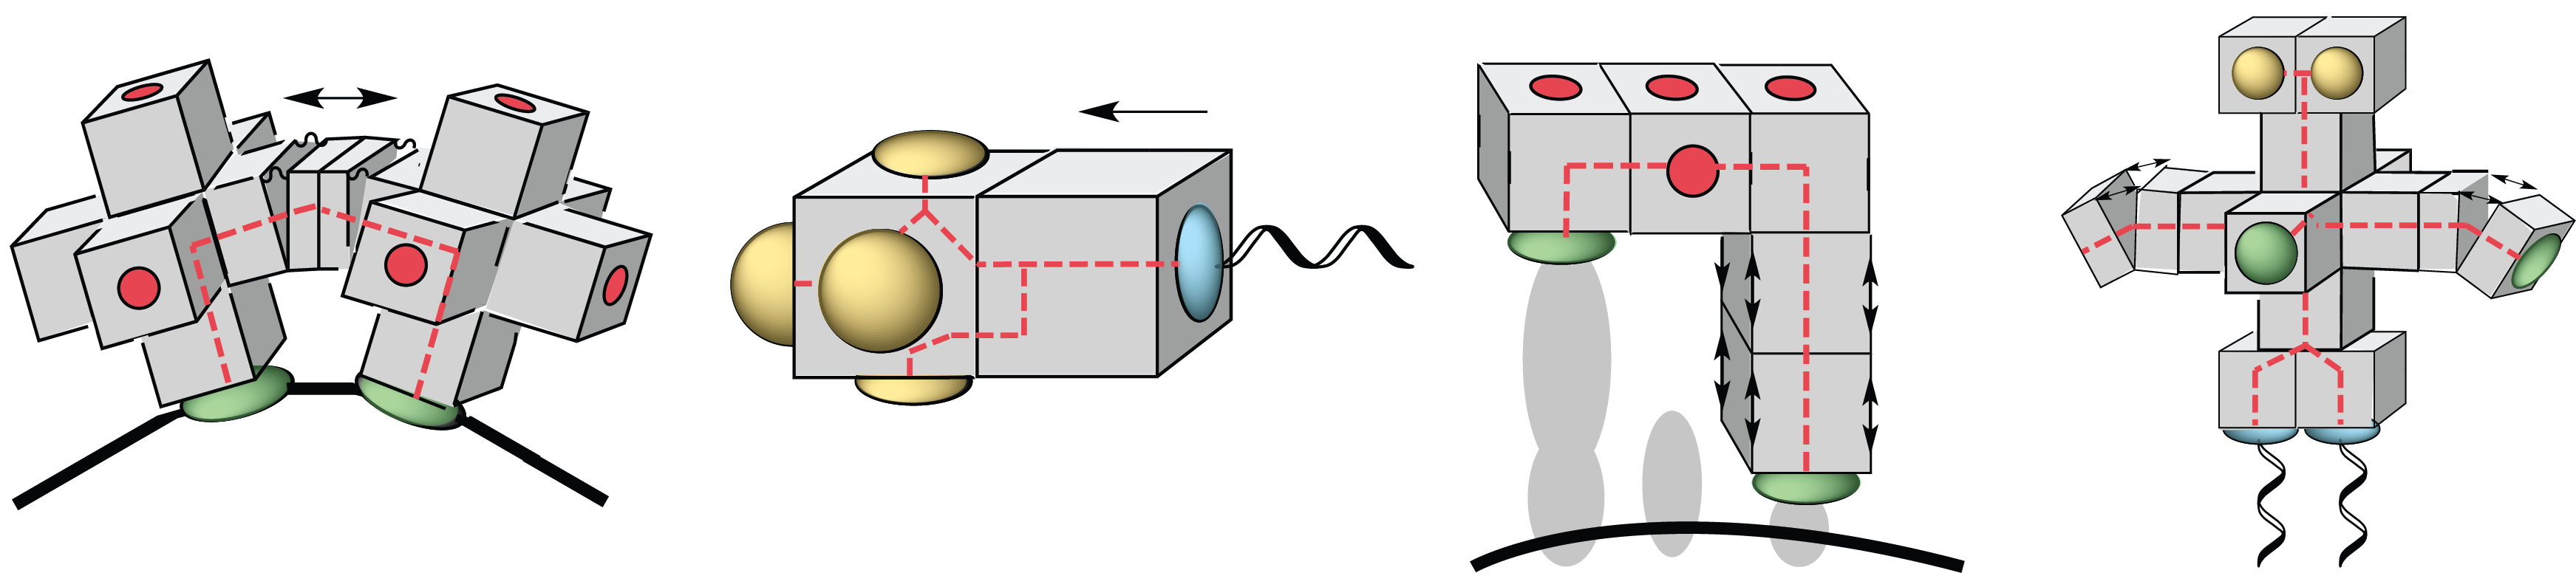
\includegraphics[width=\textwidth]{figures/dnaRoboticsHeader.png} 
    \caption{The original DNA Robotics design concept. The nanorobots are assembled from standardised cubic modules that functions as sensor, actuators, processors, or structural components. Image adapted from \url{https://dna-robotics.eu/about/}}
    \label{fig:dnaRoboticsHeader}
\end{figure}

As such, my contribution to the network and the field will be a step further in the ongoing effort to find methods for organising matter on the nanoscale.

\section{Thesis aim}
The aim of this thesis is to present methods that make it easier to design self--assembling nanostructures. This aim partly corresponds to the question of how to find the proper building blocks to use, but also how to simplify the more detailed design of individual components. The next section will cover how the results of these two topics are documented.

\section{Thesis structure}
The thesis covers two related projects, both concerning the design and modular self--assembly of nanostructures. Each project will be introduced by a separate introductory background chapter, with Chapter~\ref{ch:polycubes_intro} introducing the first project and Chapter~\ref{ch:oxview_intro} introducing the second.

\paragraph{Modular self--assembly}
The first project covers results from an abstract self--assembly model called \emph{polycubes}. Chapter~\ref{ch:polycubes_intro} provides a background to past experimental and theoretical self--assembly results. Furthermore, it includes an introduction to \emph{DNA origami}, which is also relevant for the second project. Chapter~\ref{ch:polycubes1} then details the polycube model and the shapes we get when randomly sampling the input space. Chapter~\ref{ch:polycubes2} presents the results on the inverse problem: given a polycube shape, which input rules will reliably assemble it and what is the least complex input?

\paragraph{Nucleic acid design, simulation, and visualisation}
The second project takes a more detailed view of self--assembly. Chapter~\ref{ch:oxview_intro} provides background on computer--aided design tools for nucleic acid structures, together with some related simulation models. Chapter~\ref{ch:oxview} presents my contributions to \emph{oxView}, a web--based tool for the visualisation, design, and integration of DNA, RNA and protein structures.

\paragraph{}
Finally, Chapter~\ref{ch:conclusion} discusses the results of both projects and provides some concluding remarks.

%Before moving on to the individual projects, however, the following sections will provide a general background on nucleic acid self--assembly and complexity.

%\section{Scope of the thesis}

